\chapter{Topical Community Detection in Event-based Social Network}  \label{ch:community-detection}
\graphicspath{{Part2/Chapter3/figures/}}

Websites such as   Lanyrd, Last.fm, Flickr and Twitter host an ever increasing amount of event-centric knowledge maintained by rich social interactions. In particular, there exists two types of \textit{Event-based Social Networks} (EBSN). The former is represented by the typical online activities such as sharing media and exchanging thoughts. The latter captures the face-to-face social interactions reflecting the offline co-participation in the same events. For example, in the academic conferences, researchers interact with other community members with whom they share common research background~\cite{Li:dasfa11a}. In other words, EBSN is a heterogeneous social network underlying the co-existence of both online and offline social links~\cite{Liu:KDD12}. Meanwhile, the information about these social interactions are spread over multiple websites. For example, people tend to mostly use media platforms (Flickr, Twitter) to share photos and thoughts about events, whereas they express their intent to attend events (RSVP) in online event directories (Eventful, Last.fm). Exploiting the overlap of these distributed websites is a key advantage to analyze the social networks. 

Community detection is considered as a major topic for analyzing social networks and has recently received a great attention. It aims to uncover the substructures within a network revealing which users are likely to have common interests, occupations and social properties. The information about the underlying communities can be of a great benefit for many tasks such as information diffusion and personalization. For instance, a personalization system can be based on user's community to gain more knowledge about his/her behavior~\cite{Shardanand:SIGCHI95,Paliouras:2012}. It has been also proved that the substructures within a network provide new powerful means of recommendation and collaborative filtering~\cite{Konstan:2012,Paliouras:2012}.


\section{Background} \label{sec:background}

Broadly speaking, detecting communities is dividing the vertices into groups such that there is a higher density of links within groups than between them~\cite{Clauset:PR04}. To achieve this, most of existing methods focus on network topology and structural properties. They assume that the interaction strength of users is the reflection of their proximity. However, communities detected by link-based methods often represent users having different interests since no consideration of the topical dimension was made. It is difficult to interpret the relationships of users grouped within such communities~\cite{Juan:cason11,Zhongying:12}. This problem becomes more important when users interact with objects related to diverse topics. Therefore, merging the semantic information with the linkage structure is essential in order to detect meaningful and interpretable communities. 

In EBSN, it is ideal to analyze the rich content about users and events in order to discover semantically coherent communities. Moreover, a person is naturally interested in many events which may be associated with multiple topics. It is thus more reasonable to divide users into overlapping topical groups instead of disjoint ones. Still, communities produced by topic-based methods may contain weakly connected users. They do not consider the relationships between users which results in significant loss of social information. An efficient community detection algorithm should cluster individuals who are closely connected and share common topics. 

In this chapter, we propose a novel approach to detect topical communities (i.e group of users sharing a common topic) by combining event clustering with link analysis. First, we compute the similarity of events based on the social information and the content attributes. Then, we use a hierarchical clustering to group events into different topics. Finally, a link-based function is defined to determine the effective user attachment to each community. 

%%%%%%%%%%%%%%%%%%%%%%%%%
%%%  2. Related Work  %%%
%%%%%%%%%%%%%%%%%%%%%%%%%
\section{Related Work} \label{sec:related-work-com}
Community detection has attracted attention in recent years leading to several interesting studies. Most of existing works attempt to detect disjoint communities by optimizing different link-based objectives. One popular example is the modularity optimization~\cite{Clauset:PR04,Newman:04} used to maximize the connectivity between nodes within one community and minimize the connectivity between groups. Another example is the minimization of a defined cut function in spectral methods~\cite{Scott:05}. These works mostly focused on structural properties and linkage patterns of people and they have been successfully used in some applications. However, they generally produce communities associated with different semantic topics.

To overcome the limitation of link-based methods, some studies attempt to exploit topic modeling techniques such as pLSA~\cite{Thomas:99}, LDA~\cite{Blei:MLR03} and AT (Author-Topic Model)~\cite{Steyvers:kdd04} used to detect topical communities. For example, the work in~\cite{Li:2013} made an analogy between the LDA document-topic-word and the user-topic-websites. The idea behind is that users sharing similar online access pattern tend to belong to the same topical group. This method primarily relies on the link information in a social graph, and it is only efficient when regular interaction patterns can be detected. Another technique called Community-User-Topic (CUT)~\cite{Zhou:WWW06} extends the LDA model to detect communities using the semantics of content. As a result, communities are represented as random mixtures over users who are associated with a topical distribution. This method does not consider the link information assuming that community members only share  common topics. Obviously, both methods can not be applied in real-world social networks where users' memberships are conditioned on their social relationships as well as their shared interests~\cite{Zhongying:12}.

Recently, some works start to investigate the combination of both content and link information. For example, the generative Bayesian model (Topic User Recipient Community Model) presented in~\cite{Sachan:WWW12} combines discussed topics, interaction pattern and network topology to detect topical communities. In~\cite{Zhongying:12}, Zhao et al. proposed an approach based on a modified k-means algorithm (EWKM-Entropy Weighting K-means) to partition social objects (e.g. mails, events, etc). into topical clusters. Each topical cluster contains members who interacted with the associated social objects. Then, a modularity maximization method is employed in each topical cluster to detect strongly connected communities. In our work, we made analogy between these social objects and events and we extensively compare our algorithm with this approach (called EWKM-based method in the following). 

The last concern in related work is the research on discovering communities in EBSN. Liu et al.~\cite{Liu:KDD12} addressed the problem of community detection in heterogeneous network. Their approach is based on an extended Fiedler method to consider both the online and offline social interactions. This method seems efficient to detect cohesive communities, but it is still a link-based method and no interpretation of detected communities was made. In~\cite{Li:dasfa11a}, the Event-based Community Detection (ECODE) algorithm enriched the network with virtual links based on content-based users' similarity. Virtual links aim to enhance connectivity among individuals sharing common topics (e.g. content). A hierarchical clustering is then used to group events based on their physical and virtual similarity. In the same context, Wang et al.~\cite{Wang:14}, proposed a community detection approach in location-based social network (LBSN). Their approach exploits different features such as user social similarity and venue-user similarity, and uses an edge-centric co-clustering which simultaneously discovers overlapping groups of venues and that of users. To sum up, these different studies provide important insight into detecting communities in EBSN. However, none of them aims to maximize both connectivity strength and topical purity within communities.


%%%%%%%%%%%%%%%%%%%%%%%%%%%%%%%%%%%%%%%
%%%  Event-based Social Network  %%%
%%%%%%%%%%%%%%%%%%%%%%%%%%%%%%%%%%%%%%%
\section{Event-based Social Network} \label{sec:esbn}
In this section, we describe how to construct an event-based social network using offline and online interactions (Section \ref{sec:esbn-def}) and we highlight some of their interesting properties (Sections \ref{sec:spatial-aspect} and \ref{sec:network-prop}).

\subsection{EBSN Definition}   \label{sec:esbn-def}

Based on user activities in social services, we define the following EBSNs making difference between online and offline networks. Slightly different from the definition given by Liu et al.~\cite{Liu:KDD12}, we consider that the online EBSN is constructed by solely capturing the online interactions such as sharing comments and photos about events. This online EBSN is different from the online ``friendship'' social network that may exist in some services as defined in~\cite{Liu:KDD12}. Similarly, the offline EBSN is constructed by considering the physical co-participation in social events.

\vspace{2mm}
\begin{itemize}
\item \textbf{Event Directory}
	\begin{itemize}
	\item {\textbf{Last.fm EBSN.}} In Last.fm, there are two networks: the online EBSN is built based on the online co-commenting of social events, whereas the offline 		EBSN is based on the explicit RSVP provided by users.
	\end{itemize}

\item \textbf{Media Directories}
	\begin{itemize}
	\item {\textbf{Flickr EBSN.}} Flickr is one of the most important online photo sharing websites. Thus, we exploit the activity of co-sharing photos related to the same events to build an online media EBSN.

	\item {\textbf{Twitter (Lanyrd) EBSN}} Twitter is a popular micro-blogging service, and it is by far the most used back-channel for commenting scientific conferences~\cite{Khrouf:RAMSS12}. Similarly, we exploit the co-commenting activity about the same conferences to build another online media EBSN.
	\end{itemize}
\end{itemize}


\subsection{Spatial Aspect of Social Interactions}   \label{sec:spatial-aspect}
In the following, we investigate how far from their homes people interact within the offline and online EBSNs. Therefore, we compare the geographical distance between an event location and the user's home. However, as the user's home location is not explicitly provided by Last.fm, we infer it using the average of most frequent positions of attended events. Results are depicted in Figure~\ref{fig:event-user-distance} based on a random set of events and their associated users.

We observe that 95\% of users' activities in offline network are within 100 km. This rate slightly decreases in online Last.fm EBSN indicating that people tend to also comment nearby events. This aspect has already been proved in an existing study~\cite{Liu:KDD12} showing that users' activities in EBSNs are much more location constrained compared with location-based social network. In contrast, the online interactions in media-based EBSNs seem to be less conditioned on event location. The reason behind can be two-fold: (1) the nature of sharing activity which is more present in media platforms than event directories, and the users are generally non-uniformly spread; (2) the type of events indicating that people tend to travel far from their home for business purpose (conference) rather than for entertainment activity (musical concert).  

\begin{figure}[H]
  \centering
  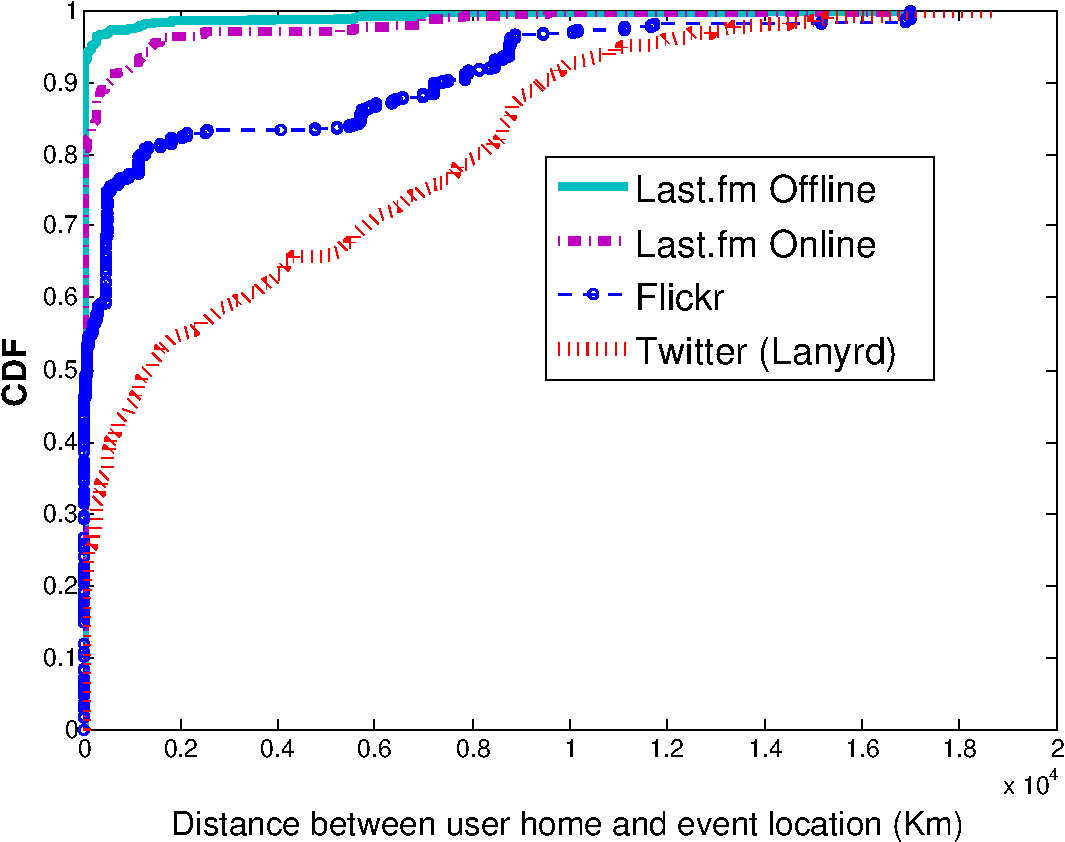
\includegraphics[scale=0.5]{location-participation.pdf}
  \caption{Locality of user activities in offline and online EBSNs}
  \label{fig:event-user-distance}
\end{figure}

Based on these findings, we decided to perform community detection using conferences from different cities in Lanyrd, whereas we only focus on a specific geographical location in Last.fm. 

\subsection{User Participation}   \label{sec:network-prop}

\begin{figure}[htb]
\centering
\subfigure[]{\label{fig:users-events_a}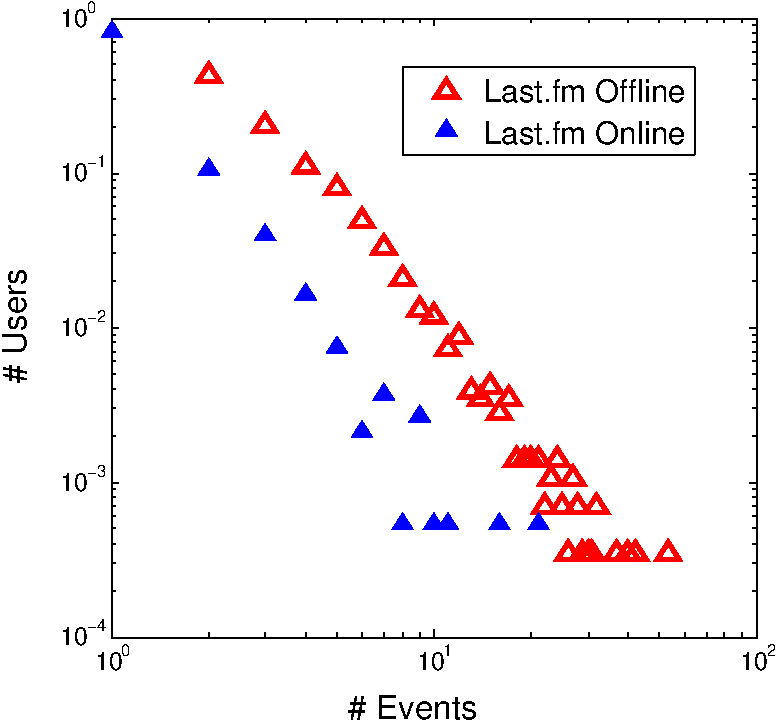
\includegraphics[height=60mm,width=67mm]{users-events-1.pdf}}
\subfigure[]{\label{fig:users-events_b}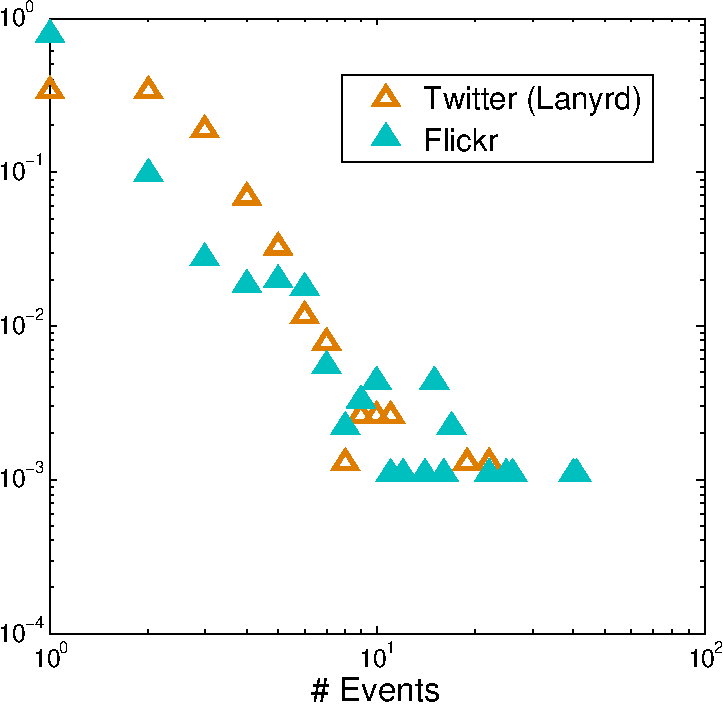
\includegraphics[height=60mm,width=63mm]{users-events-2.pdf}}
\caption{Number of participants per event in (a) Last.fm offline and online EBSN and (b) Flickr and Twitter online EBSN}
\label{fig:users-events}
\end{figure}

To gain insight into some EBSN properties, we study the user participation behavior. As shown in Figure~\ref{fig:users-events}, the results resemble a power-law distribution indicating that most of users are associated with few events. Similar results have been highlighted in other works studying the event attendance behavior~\cite{Liu:KDD12,Han:NCWTW12}. In particular, there are 81\% of users who are associated with only one event in Last.fm online EBSN, and 76\% of users sharing photos of only one event in Flickr EBSN (this can be drawn from Table~\ref{tab:dataset-stats} if we compare the number of media shared with the number of users). During the evaluation, we will show the influence of the user participation distribution on community detection.    


%%%%%%%%%%%%%%%%%%%%%%%%%%%%%%%%%%%%%%%%
%%%  4. Topical Community Detection  %%%
%%%%%%%%%%%%%%%%%%%%%%%%%%%%%%%%%%%%%%%%
\section{Topical Community Detection} \label{sec:community}
In this section, we first describe our graph model (Section~\ref{sec:modeling}). Then, we present our approach proposed to detect topical communities. 

%%%%%%%%%%%%%%%%%%%%%%%%%%
%%%  5.1 Graph Modeling %%%
%%%%%%%%%%%%%%%%%%%%%%%%%%
\subsection{Graph Modeling}  \label{sec:modeling}
Taking into account the users, the events and their related attributes, we consider the fourth-tuple graph $G=<U,S,T,E>$ for both online and offline EBSN where $U$ is the set of users, $S$ is the set of social events which are in turn associated with a set of tags, and finally $E$ is the set of undirected edges. $E$ contains two kinds of links $E=E_{US} \cup E_{UU}$:
\begin{itemize}
\item $E_{US}$ denotes the links between users and social events, formalized as $E_{US}={\lbrace(u,s)| u \in U,s \in S \rbrace}$
\item $E_{UU}$ is the set of links between users (i.e. a link represents the co-participation in same social event), formalized as $E_{UU}={\lbrace(u_{i},u_{j})| u_{i} \in U,u_{j} \in U \rbrace}$. 
\end{itemize}

In this graph, each user can be represented as a vector of events, and each event can be represented as a vector of users. Similar way is applied using the event-tag relationship. We exploit these representations to compute the similarity of events which will be used for detecting communities.

\subsection{The Proposed Approach}   \label{sec:approach}
In our approach, we follow the same rationale as the EWKM-based method proposed by Zhao et al. ~\cite{Zhongying:12}. The idea behind is to group together the social objects which share the same topic, and  . Then, users within each cluster are divided into sub groups using the modularity maximization. Instead of performing two-step clustering, we propose one step clustering taking into account both the link and content information. 

%%%%%%%%%%%%%%%%%%%%%%%%%%
%%%  5.2 Similarity Computation %%%
%%%%%%%%%%%%%%%%%%%%%%%%%%
\subsubsection{Similarity Computation}  \label{sec:similarity}
In EBSN, the overlapping communities of users who share common interests can be detected by clustering similar events together~\cite{Li:dasfa11a}. Given the large number of users, we assume that event-based clustering have a less computational time compared with user-based clustering.  Still, the event similarity should reflect both the link and content information in order to discover topical communities. To solve this, we use the notion of \emph{Homophily} which is observed in many social networks~\cite{McPherson:2001}. Homophily refers to the tendency of persons to be associated with other persons that share similar characteristics. In other words, users involved in same events have a higher likelihood to share similar interests and get connected. Similarly, tags associated with same events are more likely to be topically similar. This implies that similar events are sharing both like-minded users and semantically similar tags. Thus, we cluster events based on their similarity both in the user space and in the semantic space.

In the event-user network, events can be represented as a vector of users, and users can also be viewed as a vector of events. To reduce the dimension of the event-user matrix, we need to represent events in a latent user space using an orthogonal basis. Singular Value Decomposition (SVD) is one popular technique employed to obtain such basis.  Given a matrix $A$, the singular value decomposition is the product  $U \Sigma V^T$ where $U$ and $V$ are the left and right singular vectors and $\Sigma$ is the diagonal matrix of singular values. Event vectors in the latent user space is represented by the matrix $\tilde{A}$ as follows:

\begin{equation}  \label{eq:event-latent}
\tilde{A}=U\Sigma \Rightarrow  \tilde{A}=AV
\end{equation}
In order to detect similar events that share like-minded users, we leverage the spectral co-clustering~\cite{Dhillon:KDD01} indicating that only the top singular vectors, except of the first one, contain partition information. The algorithm first normalizes the event-user matrix as follows: 

\begin{equation}  \label{eq:event-latent}
A_n=D_1^{-1/2} A D_2^{-1/2} 
\end{equation}
where the entries of the diagonal matrices $D_{1} $ and $D_{2}$ are respectively the event degrees and the user degrees (i.e. a degree is the number of connections the node has to other nodes). Then, applying SVD on $A_n$ gives $A_n=U_n \Sigma_n V_n^T$.  Only the top-k singular vectors (except of the first one) are selected from $V_n=(v_1, v_3,...,v_n)$ to form the matrix $V'_n=(v_2, v_3,...,v_m)$ where $m \ll n$. Finally, the event representation in the user latent space is shown in Equation~\ref{eq:event-latent-1}.

\begin{equation}  \label{eq:event-latent-1}
\tilde{A}=D_1^{-1/2} A_n V'_n
\end{equation}
Similarly, we represent events in the latent semantic space applying this method on the event-tag network. Recent experiments in text corpus suggests that the dimension $m$ of $V'_n$ depends on the corpus size and it was set between 50 and 1000~\cite{Landauer:2008}. Indeed, small value of $m$ is advantageous to remove noisy information. In our case, we set $m$ equal to 200 for the user space and equal to 50 for the semantic space (there are more users than tags in our dataset). Afterwards, we use Cosine distance to compute the events similarity $S_u$ in the latent user space and $S_t$ in the latent semantic space. Finally, we combine the similarities as follows:

\begin{equation}  \label{eq:event-sim}
S_{sim} =\alpha \ S_u + (1-\alpha) \ S_t
\end{equation}
where $\alpha$ is the parameter that controls the balance between user-oriented similarity and tag-oriented similarity. In this approach, the pair-wise computation using Cosine distance can be reduced by selecting candidate solutions that only index the potentially similar events. Intuitively, these solutions are the events that share in common a minimum number of tags or users with the original event. Variants techniques can be used such as the Locality Sensitive Hashing (LSH)~\cite{Gionis:VLDB99} or its variants (e.g. MultiProbe LSH~\cite{Lv:VLDB07}) which are popular high-dimensional similarity search methods. In ECODE algorithm~\cite{Li:dasfa11a}, it has been shown that the candidate selection was efficient to save a significant amount of computational time without affecting the communities detected. Although it can be easily applied, candidate selection is not considered in the present work since we deal with small datasets.

%%%%%%%%%%%%%%%%%%%%%%%%%%
%%%  5.3 Hierarchical Clustering %%%
%%%%%%%%%%%%%%%%%%%%%%%%%%
\subsubsection{Hierarchical Clustering} \label{sec:clustering}
Inspired by the ECODE algorithm~\cite{Li:dasfa11a} described in related work (Section~\ref{sec:related-work-com}), a hierarchical agglomerative clustering is used to group similar events in terms of correlated users and tags. Agglomerative clustering begins by assigning each data item to its own individual cluster. The two most similar clusters are merged together into a single cluster.  This step is repeated until all the items are grouped into a single cluster, thus forming a hierarchy (i.e. tree).

\begin{algorithm}
\caption{Agglomerative clustering of similar events}
\label{alg:clustering}
\begin{algorithmic}
\STATE S: set of social events $s_1, s_2...s_i$
\STATE T: number of topics
\STATE $S_{sim}$: event similarity matrix
 \WHILE {Community Size$>$T \And {\  } $SemQ$ function increases}
	   \STATE Merge the most similar events $s_i$ and $s_j$ into a new event $s_{new}$
 		\FOR {each event $s_k$ $\in$ S (or candidate set)}
 			\STATE $S_{sim}(s_{new},s_k)$ =  average($S_{sim}(s_{new},s_i)$+$S_{sim}(s_{new},s_j)$)
		\ENDFOR
\STATE Compute $SemQ$		
\ENDWHILE
\end{algorithmic}
\end{algorithm}

As outlined in Algorithm~\ref{alg:clustering}, the most similar events $s_i$ and $s_j$ are clustered together forming a new event $s_{new}$. Then, we compute the similarities between $s_{new}$ and each event in the dataset or in the candidate set (if the candidate selection is considered). Finally, the clustering stops when there is no significant increase of the quality function. This approach is advantageous compared with other algorithms such as k-means since the predefined number of clusters is not required.

To produce topical clusters, the quality function of the tree follows the same rationale than Newman modularity but applied on the semantic space. Indeed, our goal is to maximize the intra-similarities and minimize the inter-similarities in the semantic space. Thus, we define a novel function called \textit{semantic modularity}. To formalize this function, we use the events similarity  $S_t$ computed in the latent semantic space in order to compute the intra-similarities (IntraSem in Equation~\ref{eq:intra}) and inter-similarities (InterSem in Equation~\ref{eq:inter}) as following:

\begin{equation} \label{eq:intra}
       {IntraSem}=\frac{1}{|C|}\sum_{C_k \in C} \frac{\sum_{i,j \in C_k, i  C_i j } S_t(i,j)}{|C_k| (|C_k|-1)} 
\end{equation}

 \begin{equation} \label{eq:inter}
      {InterSem}=  \frac{1}{|C|} \sum_{i \in C_i} \frac{\sum_{j \in C_j,  C_i \ne  C_j} S_t(i,j)^2}{M}  
\end{equation}
where C is the set of discovered clusters, and M is the number of comparisons made in inter-similarities. Finally, the semantic modularity $SemQ$ is defined as following:

 \begin{equation} \label{eq:quality}
		SemQ=IntraSem-InterSem
\end{equation}

Note that the maximal $SemQ$ provides the topical clusters of events and stop the clustering process. In meanwhile, each detected cluster keeps in mind a minimal knowledge about the link information held by the event similarity in the user space, which makes our approach different from the EWKM-based method~\cite{Zhongying:12}. 

%%%%%%%%%%%%%%%%%%%%%%%%%%
%%%  5.4 User Assignment %%%
%%%%%%%%%%%%%%%%%%%%%%%%%%
\subsubsection{User Assignment}   \label{sec:assignment}
The last step of our approach is to group together users associated with each cluster by simply using the user-event links.  As the user may participate in many events, we can generate overlapping topical communities. However, a user may be weakly involved in one topical cluster that not really reflects his/her interests. To address this problem, we propose to discover the effective user's memberships by computing his/her assignment scores. If the user $u_i$ is a member of the community $C_i$, the assignment function is defined as follows:

\begin{equation}    \label{eq:assignment}
			AS(u_i,C_i)=\frac{D_c(u_i)}{D(u_i)}				
\end{equation}
where $D_c(u_i)$ is the degree of the user $u_i$ within the community $C_i$ (i.e. number of links of the user with other community members), and $D(u_i)$ is the global $u_i$'s degree. The user's membership to one community is determined if the related assignment score is higher than the average of non-zeros scores over all communities. Note that the user assignment method based on Equation~\ref{eq:assignment} may convert a cluster to an empty one. We believe that the removal of these empty clusters is reasonable since they represent groups of very weakly connected users.

%%%%%%%%%%%%%%%%%%%%%%
%%%  5. Experiments and Evaluation %%%
%%%%%%%%%%%%%%%%%%%%%%
\section{Evaluation}   \label{sec:experiments}
This section presents the evaluation of the proposed community detection approach applied on real-world datasets. We first describe these datasets  followed by the description of the performance metrics and the obtained results.

%%%%%%%%%%%%%%%%%%%%%%%%%%%%%%%%%%
%%%  5.1 Experimental Datasets %%%
%%%%%%%%%%%%%%%%%%%%%%%%%%%%%%%%%%
\subsection{Experimental Datasets}
Based on the definition of online and offline EBSNs, we use the following datasets placed online\footnote{\url{http://www.eurecom.fr/~khrouf/esbn}} (some statistics are shown in Table~\ref{tab:stats}).

\begin{itemize}
\item \textbf{Entertainment (Last.fm and Flickr):} We previously demonstrated that a very high fraction of social interactions for entertainment purpose  exist between geographically close friends. Hence, we focus our analysis on events located in one city. The capital ``London'' has been selected since it exhibits a significant number of users and events compared with other cities in EventMedia. Operationally, we query the EventMedia SPARQL endpoint to retrieve data, and we crawl additional metadata using the REST API of Last.fm and Flickr. Then, we pre-process the dataset as follows: First, we remove the tags associated with very low frequency (less than 5) to reduce the topical noise, and we only keep the events which are associated with the frequent tags (musical genres). Second, we remove the singletons of event-user pairs where the event has only one participant, and this participant is associated with only one event. We retrieve the events happened in 2012 and 2013 (associated with media) and we obtain the following EBSNs: (1) an offline Last.fm EBSN containing 915 events, 2847 users and 272 tags; (2) The associated online Last.fm EBSN contains 470 events (among 915 events), 1729 users and 248 tags (among 272 tags); (3) The associated online Flickr EBSN contains 375 events, 868 users and 221 tags. Note that the removal of singletons event-user pairs has significantly reduced the size of the online Last.fm and Flickr EBSNs indicating that users' activities in those networks are more sporadic and mostly present individual behaviors.

\item \textbf{Conference (Lanyrd and Twitter)} Similarly, we use SPARQL queries to retrieve data from EventMedia along with the Twitter API for additional information (e.g. user's home location). Note that Lanyrd also provides details about the conference attendees, but this information was missing in EventMedia at the time of writing. Thus, we plan to further enrich our dataset and we left the analysis of offline Lanyrd EBSN for future study. Then, we pre-process the data retrieved as follows: As no tags were associated with events, we automatically process the conference description (tokenization, stop-words removal, etc.). However, this method produced very noisy tags because some conferences are vaguely described (e.g \emph{The World is Changing, Is Your Company on Board?}).  We also attempt to automatically process the tweets. Still, many tags do not really reflect what is the conference about due to the presence of several noisy tweets (e.g. personal status updates, opinions, etc.). As an alternative solution, we manually label the conferences descriptions by selecting the most representative keywords. Due to the manual effort, we only keep the interesting conferences which are related with very active users. Finally, we obtain an online EBSN which contains 275 events, 768 Twitter users and 166 tags. Note that there is a small set of events compared with Last.fm EBSN due to the high selectivity followed.
\end{itemize}
\begin{table}[H]
\centering{
\begin{tabular}{cccc}
\hline
& Edges & Density & ClustCoeff \\
\hline
Last.fm Offline & 95897 & 0.0237 & 0.1144\\
\hline
Last.fm Online & 9936 & 0.0067 & 0.398\\
\hline
Flickr Online &  7071 & 0.0188 & 0.2624 \\
\hline
Twitter Online & 14237 & 0.0483  & 0.4852 \\
\hline
\end{tabular}
\caption{Some statistics about the datasets}
\label{tab:stats}
}
\end{table}

\subsection{Topic Modeling}
In order to assess the topical purity in each cluster, we first need to detect the set of topics in each dataset. Thus, we decided to employ LDA~\cite{Blei:MLR03}, a popular topic modeling technique where we consider the events as documents. The use of LDA has led to coherent topics in Lanyrd dataset, but slightly ambiguous topics in Last.fm datasets. We explain this difference by the manual labeling in Lanyrd dataset where we carefully select qualitative tags. In contrast, Last.fm contains crowdsourced tags generated without moderator oversight and known to be less accurate. Moreover, the musical concerts may feature many artists related to different genres (i.e topics) or only one genre, making more difficult to detect co-occurrences. The conferences, on the other hand,  often target only one major topic (e.g. Semantic Web). 

To solve the topic modeling in Last.fm, we resolved to exploit the classification of musical genres that may help detect the fuzzy similarity between them (e.g. death metal and deathcore). More precisely, we leverage the existing SKOS taxonomy\footnote{\url{http://dbpedia.org/page/Category:Musical_subgenres_by_genre}} in DBpedia using the generalization relations such as \texttt{skos:broader} and \texttt{skos:narrower}. Tables \ref{tab:topics-lanyrd} and \ref{tab:topics-lfm} show few examples of topics detected respectively in Lanyrd and Last.fm. Note that we obtained 24 topics in Last.fm consisting of high-level musical genres, and 30 topics in Lanyrd where the optimal number of topics is determined based on the approach proposed by Griffiths et al.~\cite{Griffiths:04}. Finally, Figure~\ref{fig:event-topic} shows that many conferences have at most two topics, while this number slightly increases in musical events. 

\begin{table}[H]
\centering{
\begin{tabular}{c|c}
\hline
    \textbf{Topic}       &  \textbf{Example of Lanyrd Tags}  \\
\hline
   Education  &   learning, education, teaching, technology\\
\hline
   programming  &   programming, language, python, library\\
\hline
   Innovation  &   creativity, technology, business, future\\
\hline
   Application  &   mobile, application, web \\
\hline
\end{tabular}
\caption{Example of topics detected in Lanyrd}
\label{tab:topics-lanyrd}
}
\end{table}

\begin{table}[H]
\centering{
\begin{tabular}{c|c}
\hline
    \textbf{Topic}       &  \textbf{Example of Last.fm Tags}  \\
\hline
   Heavy metal  &   metal alternative, progressive metal... \\
\hline
   Pop  &   synthpop, powerpop, pop punk...\\
\hline
   Electronic  &   indietronica, synthpop, folktronica...\\
\hline
   Rock  &    hard rock, alternative rock, glam rock... \\
\hline
\end{tabular}
\caption{Example of topics detected in Last.fm}
\label{tab:topics-lfm}
}
\end{table}


\begin{figure}[H]
  \centering
  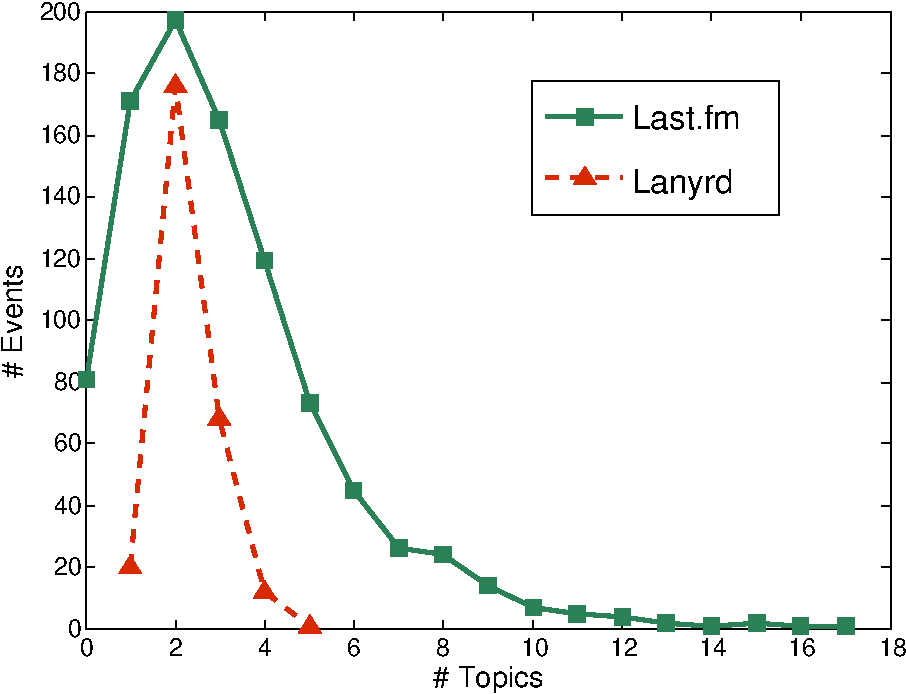
\includegraphics[scale=0.5]{topic-distrib.pdf}
  \caption{Histogram of the number of topics per event}
  \label{fig:event-topic}
\end{figure}


%%%%%%%%%%%%%%%%%%%%%%%%%%%%%%%
%%%  5.2 Performance Metrics %%%
%%%%%%%%%%%%%%%%%%%%%%%%%%%%%%%
\subsection{Evaluation Metrics}
To evaluate our approach, the performance metric should take into account the combination of both content and link information. We adopt the $PurQ_\beta$ metric introduced by Zhao et al.~\cite{Zhongying:12}. It has been inspired by the F-score measure that considers both the precision and the recall metrics. $PurQ_\beta$ considers both the topical purity and the members connectivity. First, we introduce the function that measures the topical purity in each cluster as following:

\begin{equation}    \label{eq:purity}
     Purity_i= max_j \left( \frac{n_{ij}}{n_i} \right)
\end{equation}
where $n_{ij}$ is the number of tags belonging to topic $j$ and cluster $i$, and $n_i$ is the number of tags in the cluster $i$. The final score of $Purity$ is the overall average of all the purity scores. Yet, we observed during the experiments that Purity does not effectively reflect the presence of clusters having low topical purity. Hence, we decided to also examine the $F_{purity}$ which is the faction of clusters having $Purity_i$ higher or equal than the average $Purity$. Finally, the metric $PurQ_\beta$ combining the content and link information is:


\begin{equation}    \label{eq:purq}
	PurQ_\beta= \frac{(1+\beta^2) (Purity \cdot Q )}{\beta^2 Purity + Q}			
\end{equation}
where $Q$ is the Newman modularity~\cite{Newman:04} used to evaluate the goodness of a partition, ensuring that there are many edges within communities and only a few between them. Then, the parameter $\beta$ is used to adjust the weight of $Purity$ and $Q$. $\beta=0.5$ means that $PurQ_\beta$ puts more emphasis on $Purity$ than $Q$. In contrast, $\beta=2$ puts more emphasis on $Q$. The general behavior of communities is when $Purity$ increases, $Q$ decreases, and vice versa.


%%%%%%%%%%%%%%%%%%
%%%  Results    %%%
%%%%%%%%%%%%%%%%%%

\subsection{Results} 
We first evaluate how the coefficient $\alpha$ in Equation~\ref{eq:event-sim} affects the performance of our approach. Figure~\ref{fig:alpha-impact} shows the evolution of the $Purity$ and the modularity $Q$ when $\alpha$ increases. It can be seen that the modularity increases if a high weight is assigned to event similarity in the user space. However, the purity and the modularity do not evolve at the same scale. While $Q$ slightly increases, $Purity$ drastically decreases. Thus, good values of $PurQ_\beta$ can be obtained when $\alpha \in $[0.1,0.5]. 

Then, we compare our approach with some related works: (1) Edge co-clustering (or EdgeCluster) inspired by the approach applied on the location-based social network and proposed in~\cite{Wang:14}. For this approach, we consider as features the user similarity in the event space and in the semantic space. Based on these features, Edge co-clustering uses k-means to cluster similar ``user-event'' edges. This method was evaluated only on two datasets as it requires a very large computation time; (2) ECODE algorithm which introduces the concept of content-based virtual links in the user-event graph and clusters together similar events sharing high physical and virtual links; (3) The popular Newman Modularity maximization (link-based method); (4) The EWKM-based method as detailed in related work (Section~\ref{sec:related-work-com}).

\begin{figure}[htpb]
  \centering
  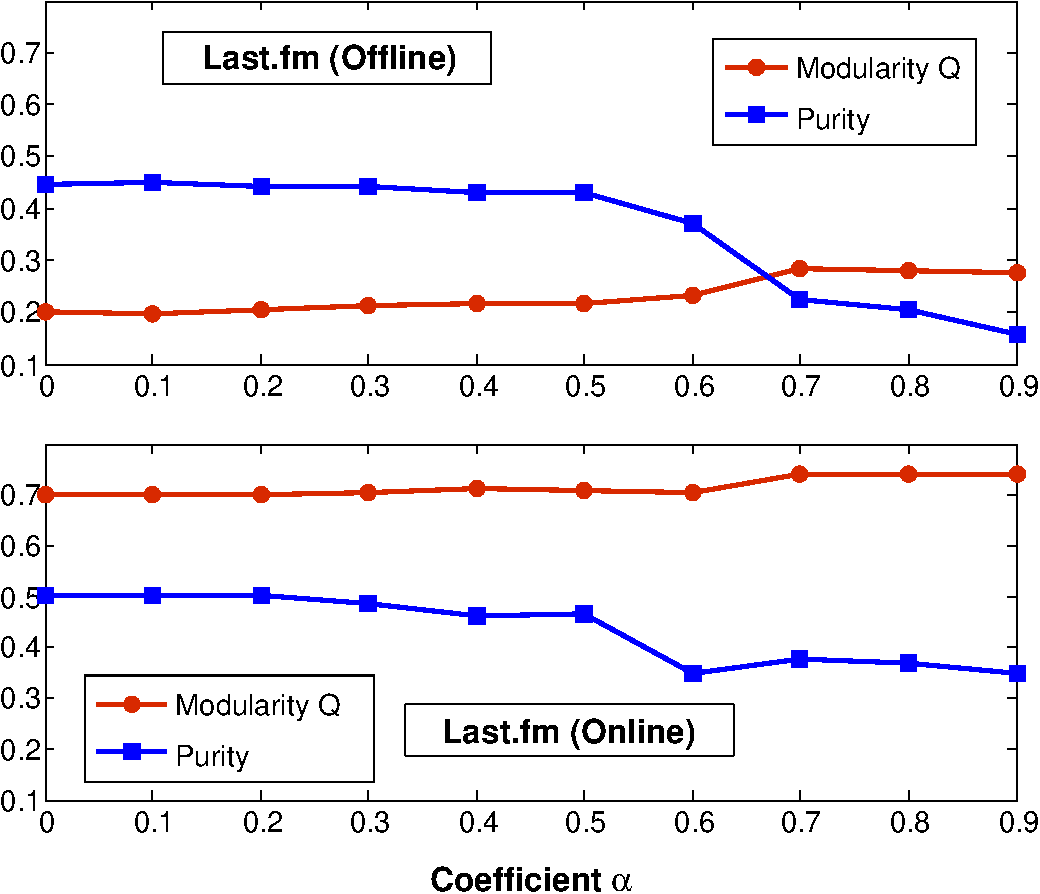
\includegraphics[scale=0.42]{alpha-performance.pdf}
  \caption{The evolution of Q and Purity with $\alpha$}
  \label{fig:alpha-impact}
\end{figure}

\begin{figure}[htbp]
  \centering
  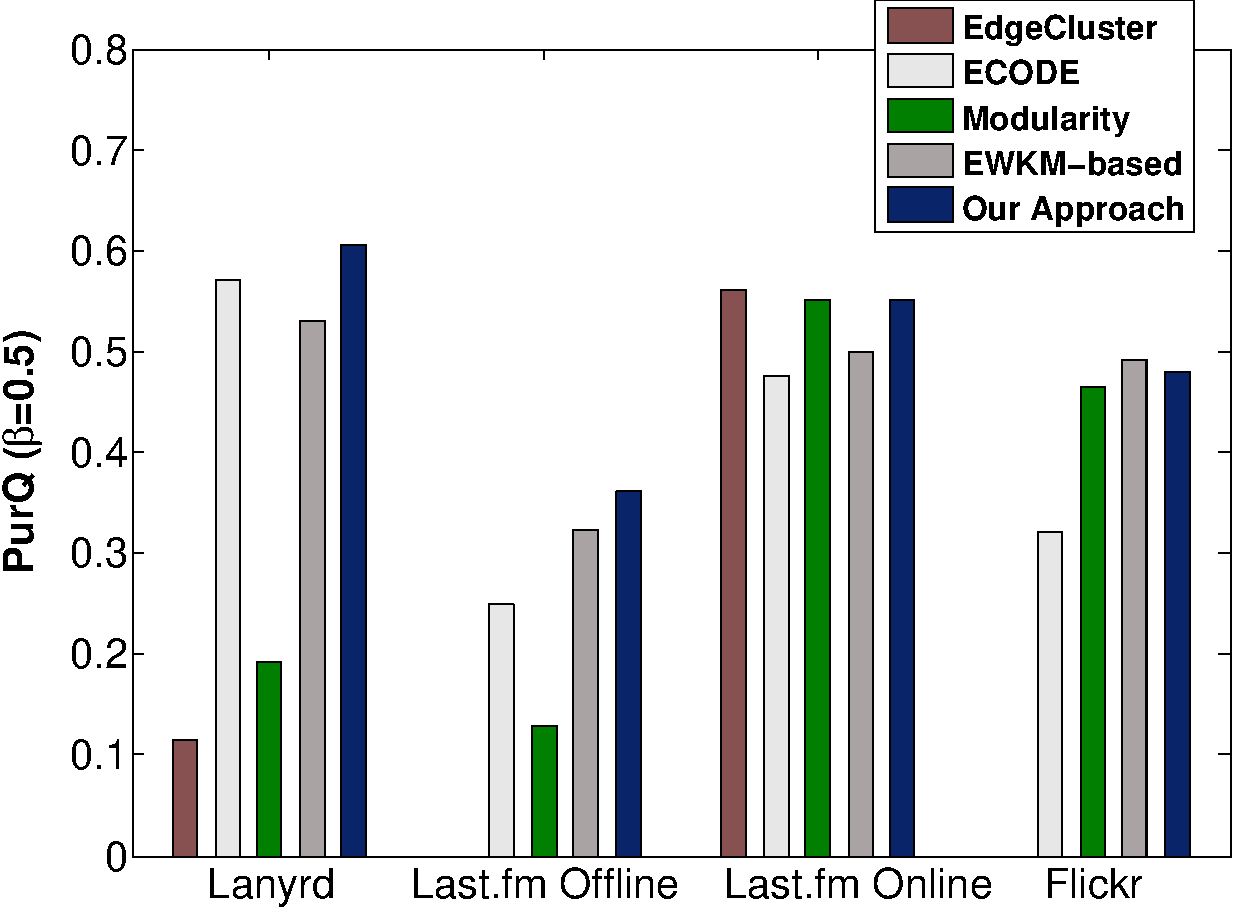
\includegraphics[scale=0.35]{PurQ-05.pdf}
   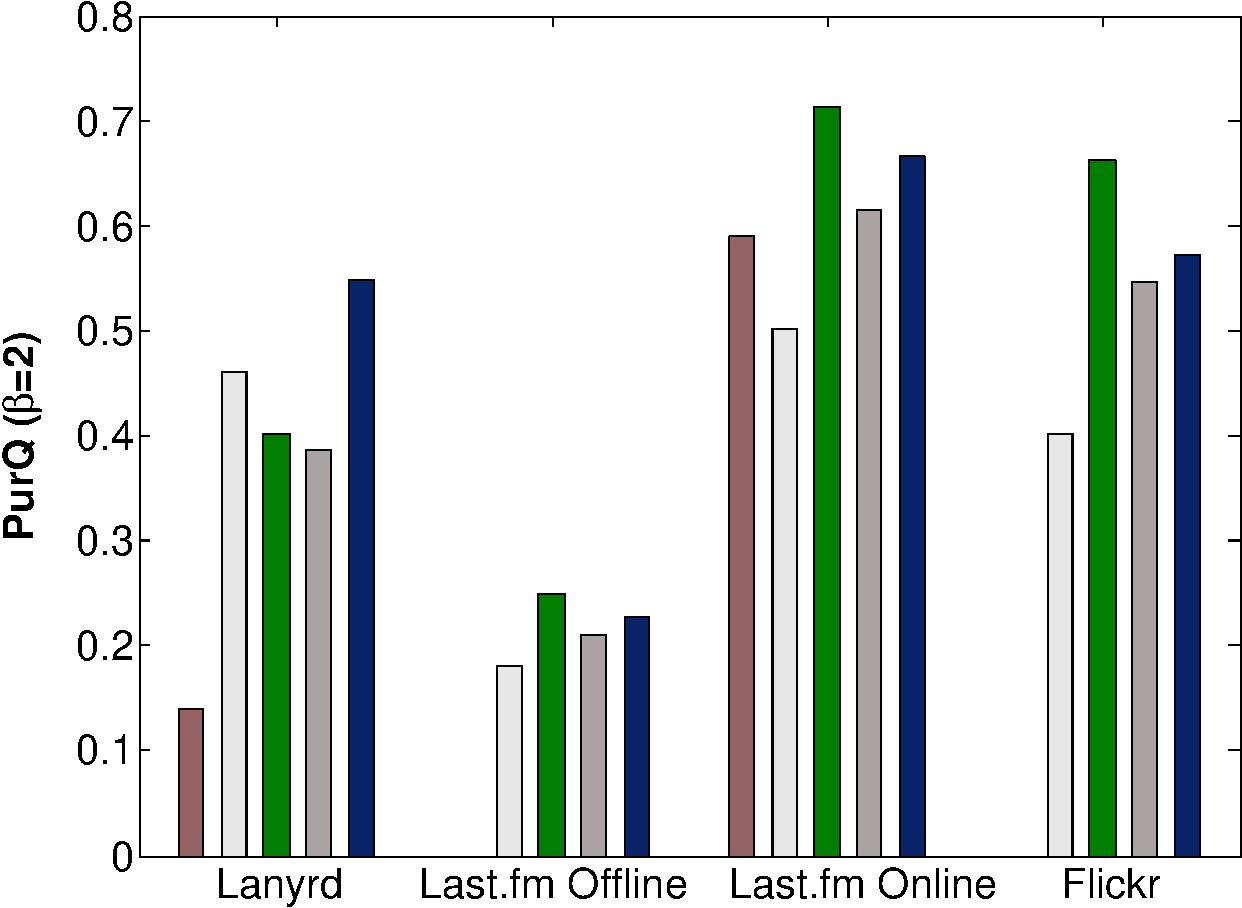
\includegraphics[scale=0.35]{PurQ-2.pdf}
  \caption{The performance comparison with $\beta=0.1$ and $\beta=2$ for different datasets}
  \label{fig:PurQ}
\end{figure}


The comparison results are depicted in Figure~\ref{fig:PurQ}. All these methods have nearly similar performance in Last.fm Online EBSN particularly when $\beta=0.5$. Indeed, the communities detected within this network have very small sizes (e.g average size equal to 15 for the Modularity method) due to the extremely sporadic interactions. This is also explained by the low density link and the user participation behavior where 92\% of users are associated at most with only two events. Hence, the link information was sufficient to obtain a good purity. This aspect slightly decreases in Flickr dataset where 78\% of users are associated with at most two events. The Modularity method apparently achieves a good purity. However, the fraction $F_{purity}$ is only equal to 0.6, a fair value compared with EWKM-based method and our approach where $F_{purity}$ are respectively equal to 0.89 and 0.91. In Last.fm Offline and Twitter EBSNs, the Modularity method has a poor performance when $\beta=0.5$. This can be explained by the network density which is high in those datasets compared with others. Moreover, the identified communities are very large. For example, we found an average size of 474.5 in the communities produced by the Modularity method in Last.fm offline EBSN. This indicates that users within this network are densely linked which can justify the low $Q$ values produced by different approaches. 


Evaluating the content-based methods, we note a better performance for ECODE in Twitter EBSN than in the other datasets. This is due to the addition of virtual links to the graph based on the content-similarity between users. However, the user profile in Last.fm is much more topically diverse than in Lanyrd which leads to ambiguous similar scores. In reality, the user may be interested in many musical concerts having different topics, whereas he has more restrictive ``scientific'' interests that mostly fit his/her expertise domain. We also observe a poor performance of the Edge co-clustering algorithm in Twitter EBSN because it is sensitive to the number of clusters that needs to be accurately determined. Finally, our approach achieves the best performance both when $\beta=0.5$ and $\beta=2$. Note that there is similar behavior between our method and the EWKM-based method. For instance, the average size of communities in Last.fm Offline EBSN is equal to 0.33 for EWKM-based, and 0.29 for our approach. However, the EWKM-based method is based on k-means clustering which is sensitive to the initial distribution of centroids, thus producing different results in each run. This problem is absent in our approach which is based on hierarchical clustering. From the computation point of view, we observe that all methods have nearly the same computational time except of the Edge co-clustering method. Finally, low purity values are observed in Last.fm Offline EBSN compared with Twitter EBSN. The reason of this lower performance is that the musical concerts are attached to much more topically diverse tags than the conferences in Lanyrd. In the following, we select the EWKM-based method to further evaluate our approach.

\paragraph{Coductance Comparison} \mbox{}\\

\begin{figure}[htb]
\centering
\subfigure[]{\label{fig:conductance_a}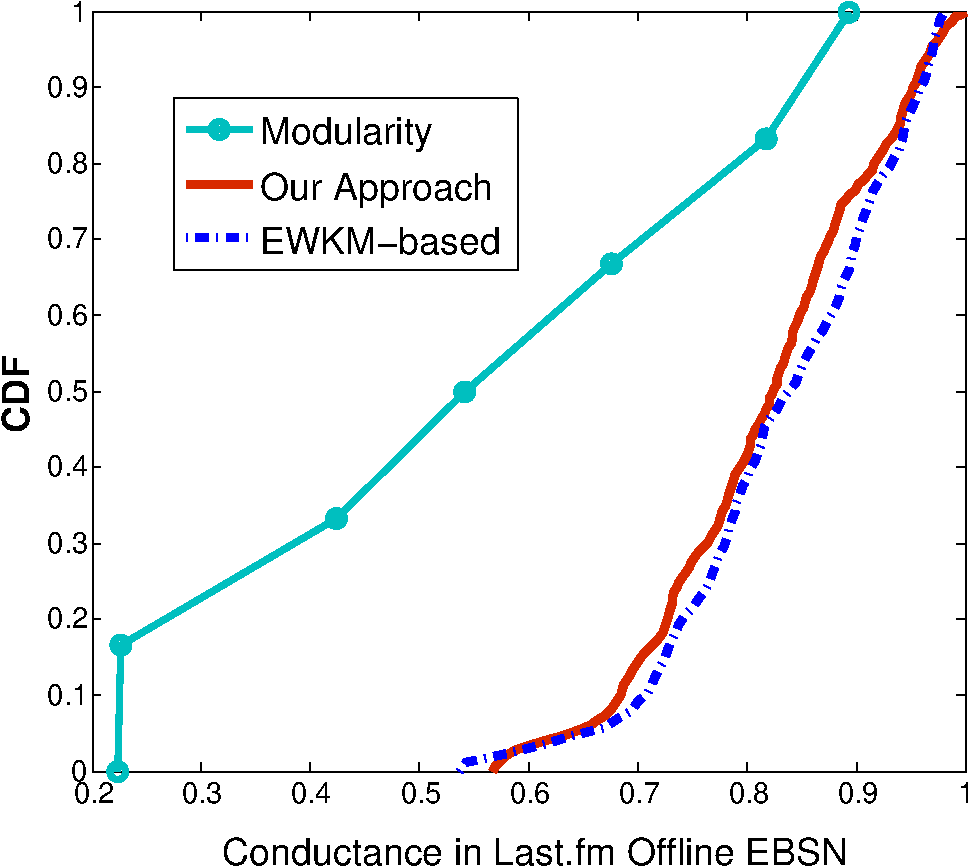
\includegraphics[height=60mm,width=67mm]{conductance-offline.pdf}}
\subfigure[]{\label{fig:conductance_b}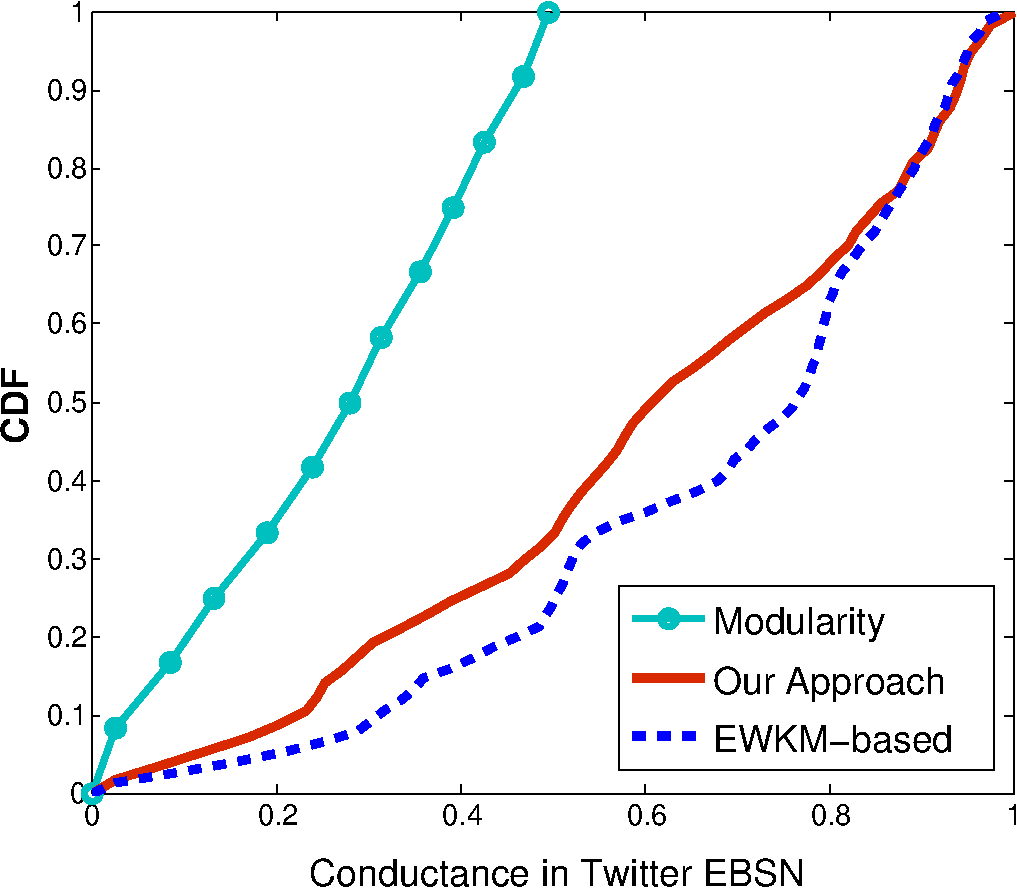
\includegraphics[height=60mm,width=63mm]{conductance-lanyrd.pdf}}
\caption{Conductance comparison in (a) Last.fm Offline EBSN and (b) Twitter EBSN}
\label{fig:conductance}
\end{figure}

It is difficult to construct a ground truth that represents the real communities within a network. Hence, we evaluate the proposed approach using the \emph{Conductance} metric~\cite{Leskovec:WWW08}. Conductance is a popular quality function assessing whether the detected communities are densely linked but weakly attached to the rest of the network. Note that this metric will evaluate our method from the link-based perspective. Lower conductance values mean better community structure. Figure~\ref{fig:conductance} shows the cumulative distribution (CDF) of the conductance respectively in Twitter EBSN and Last.fm Offline EBSN. Our approach produces slightly more communities with lower conductance values especially in Twitter EBSN. The reason behind is the strategy to determine users' memberships based on their global degrees. We believe that the better performance in Twitter EBSN is due to its clustering coefficient which is larger than that of Last.fm Offline EBSN.

\myparagraph{User Profiles Comparison} 
To evaluate our approach from the content-based perspective, one way is to compare the user profiles within one community. Hence, we retrieve the users' tags from each website and we only keep the frequent ones, thus creating a user profile. Cosine distance is then applied to compute the similarity between users' profiles. We consider that two users are similar when they have a Cosine distance above 0.3, a quite reasonable value considering the noisy tags. Figures~\ref{fig:comp-user} shows the CDF of the fraction of similar users within the same communities. It can be seen that our approach clustered more ``topically'' similar users than the EWKM-based method did. 


\begin{figure}[htb]
\centering
\subfigure[]{\label{fig:comp-user_a}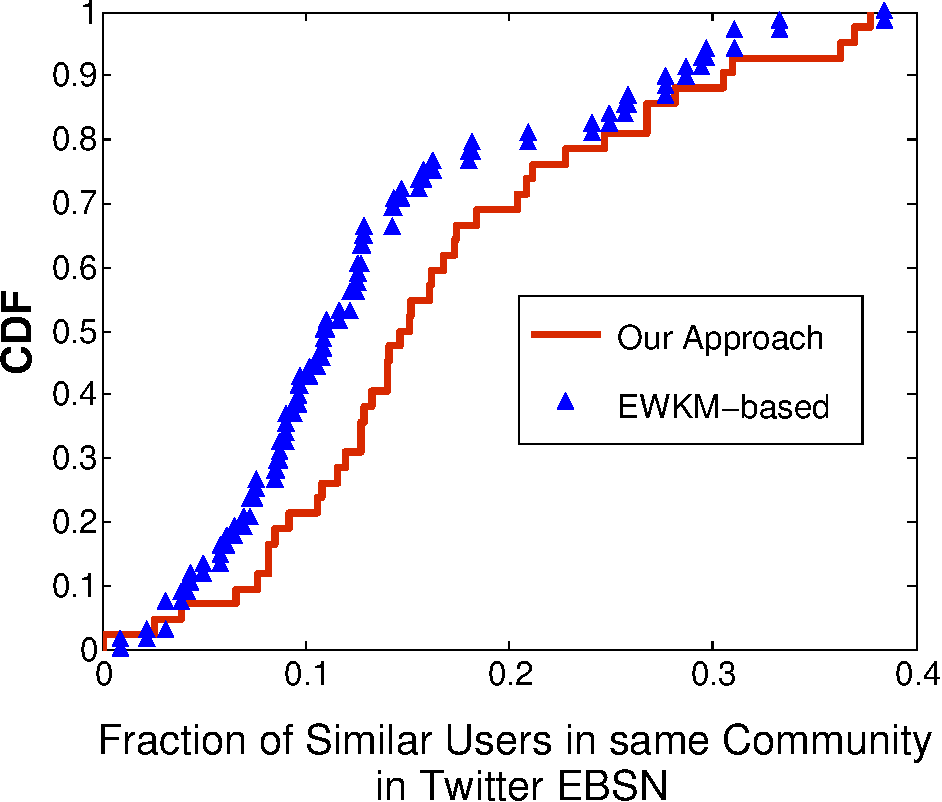
\includegraphics[height=63mm,width=68mm]{users-sim-lanyrd.pdf}}
\subfigure[]{\label{fig:comp-user_b}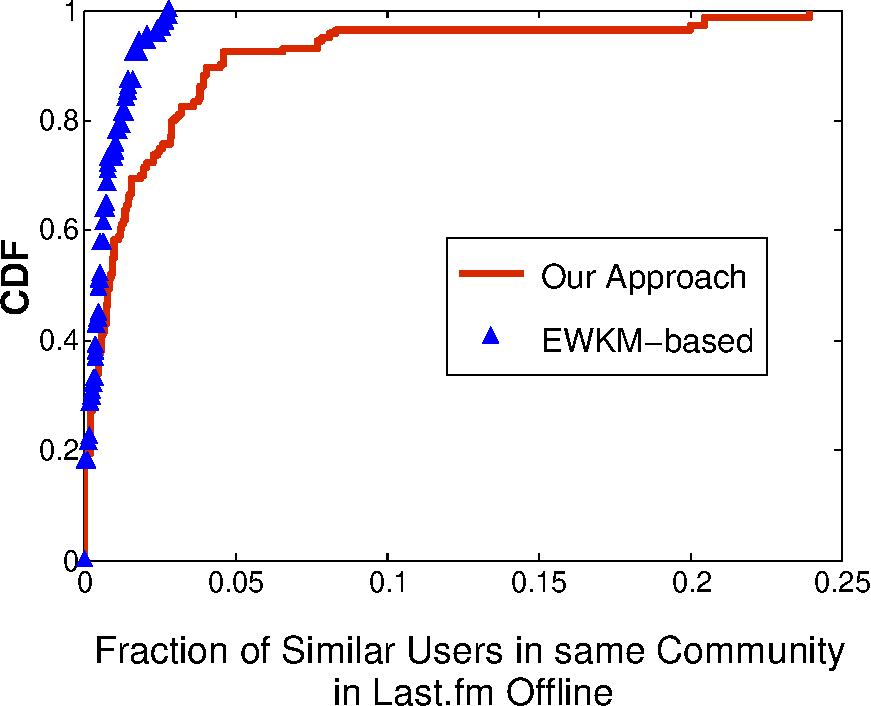
\includegraphics[height=64mm,width=68mm]{users-sim-offline.pdf}}
\caption{Comparison of user profiles in (a) Twitter EBSN and (b) Last.fm Offline EBSN}
\label{fig:comp-user}
\end{figure}

We also examine the fraction of ``friends''  within each community. The friendship information was extracted using the online social networks that exist in Last.fm and Twitter detected by our approach. Results are shown in Table~\ref{tab:friends}. We can see that a large fraction of friends were clustered in the same community by the Modularity method in Last.fm Offline EBSN compared with the other methods. This is also justified by the very high average size of communities detected which is equal to 474.5. Moreover, it is clearly shown that the conference attendees having similar topical interests are more likely to be friends than the case of concert attendees. 

\begin{table}[H]
\centering{
\begin{tabular}{ccc}
\hline
    \textbf{Method}    &   Twitter (Lanyrd) & Last.fm Offline \\
\hline
   Modularity-based  &  0.72 & 0.69\\
\hline
   EWKM-based  &   0.70 &0.23\\
\hline
   Our Approach  & 0.73   & 0.29\\
\hline
\end{tabular}
\caption{Average fraction of friends within communities}
\label{tab:friends}
}
\end{table}

\myparagraph{Communities Overlap} 

\begin{figure}[htb]
  \centering
  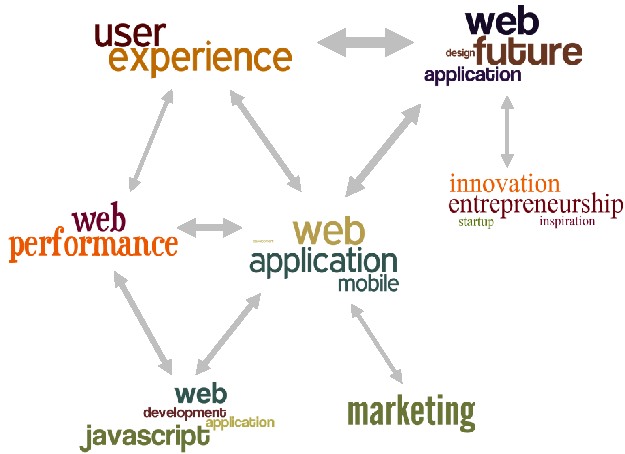
\includegraphics[scale=1]{tagCloudLanyrd.pdf}
  \caption{A sample of some overlapping communities in Twitter EBSN}
  \label{fig:tagcloud}
\end{figure}

Lastly, Figure~\ref{fig:tagcloud} shows a tag cloud representing a sample of the most overlapping communities in Twitter EBSN. The link thickness exhibits the overlapping degree. It can be drawn that the main topic of these communities is the Web domain which is the interest of many users who share different ``topical'' expertise. 

In Twitter EBSN, our approach detects 65 communities while the EWKM-based method produces 92 communities. Analyzing both community structures, it is found that our approach discovers fewer but more cohesive topical communities. We evaluate the cohesiveness using the popular Silhouette coefficient~\cite{Rousseeuw:1987}. For instance, we have detect only one community about the topic ``\emph{user experience}'' with a cohesion equal to 0.1. In contrast, 4 communities have been detected about this topic by the EWKM-based method including  2 singletons  (i.e. community having one user)  and having a cohesion equal to -0.3. This finding underlines the advantage of our approach to group together strongly linked users and to remove communities having weak connectivity.

\section{Conclusion}   \label{sec:conclusion}
Today's people use event and media websites to interact together either online by sharing comments and photos or offline by attending events. Thus, many social connections can be formed and strengthened during social events which can be considered as a basis to detect communities. In this chapter, we proposed a new approach to discover topical communities from event information. Taking into account both the content and the link information, we clustered events by maximizing a newly defined metric called \emph{Semantic Modularity}. Then, the user membership to each cluster was determined by a link-based function based on the user's degree. A comparison with existing studies shows the efficiency of our approach to detect communities optimizing both users connectivity and topical purity. Results highlighted how people interact differently in offline and online EBSN and how these interactions depend on the event category (e.g conference, concert, etc.). For future work, we plan to combine both the offline and the online worlds to solve community detection in a heterogeneous network. We wish to assess the impact of such combination on the purity and the connectivity of topical communities.